% Adjust these for the path of the theme and its graphics, relative to this file
%\usepackage{beamerthemeFalmouthGamesAcademy}
\usepackage{../../beamerthemeFalmouthGamesAcademy}
\usepackage{multimedia}
\graphicspath{ {../../} }

% Default language for code listings
\lstset{language=C++,
	morekeywords={each,in,nullptr}
}

% For strikethrough effect
\usepackage[normalem]{ulem}
\usepackage{wasysym}

\usepackage{pdfpages}

% http://www.texample.net/tikz/examples/state-machine/
\usetikzlibrary{arrows,automata}

\usepackage{qtree}


\newcommand{\modulecode}{GAM250}\newcommand{\moduletitle}{Advanced Games Programming }\newcommand{\sessionnumber}{2}

\begin{document}
\title{\sessionnumber: AI}
\subtitle{\modulecode: \moduletitle}

\frame{\titlepage} 

\begin{frame}
	\frametitle{Learning outcomes}
	\begin{itemize}
		\item \textbf{Understand} navigation in Video Games
		\item \textbf{Implement} Finite State Machines in Unity
		\item \textbf{Implement} Behaviour Trees in Unity
	\end{itemize}
\end{frame}

\part{Pathfinding}
\frame{\partpage}

\begin{frame}{The problem}
    \begin{itemize}
        \item We have a \textbf{graph} \pause
            \begin{itemize}
                \item \textbf{Nodes} (points) \pause
                \item \textbf{Edges} (lines between points, each with a \textbf{length}) \pause
            \end{itemize}
        \item E.g.\ a road map \pause
            \begin{itemize}
                \item Nodes = addresses \pause
                \item Edges = roads \pause
            \end{itemize}
        \item E.g.\ a tile-based 2D game \pause
            \begin{itemize}
                \item Nodes = grid squares \pause
                \item Edges = connections between adjacent squares \pause
            \end{itemize}
        \item Given two nodes $A$ and $B$, find the \textbf{shortest path} from $A$ to $B$ \pause
            \begin{itemize}
                \item ``Shortest'' in terms of edge lengths --- could be distance, time, fuel cost, ...
            \end{itemize}
    \end{itemize}
\end{frame}

\begin{frame}{Applications of pathfinding}
    \begin{center}
        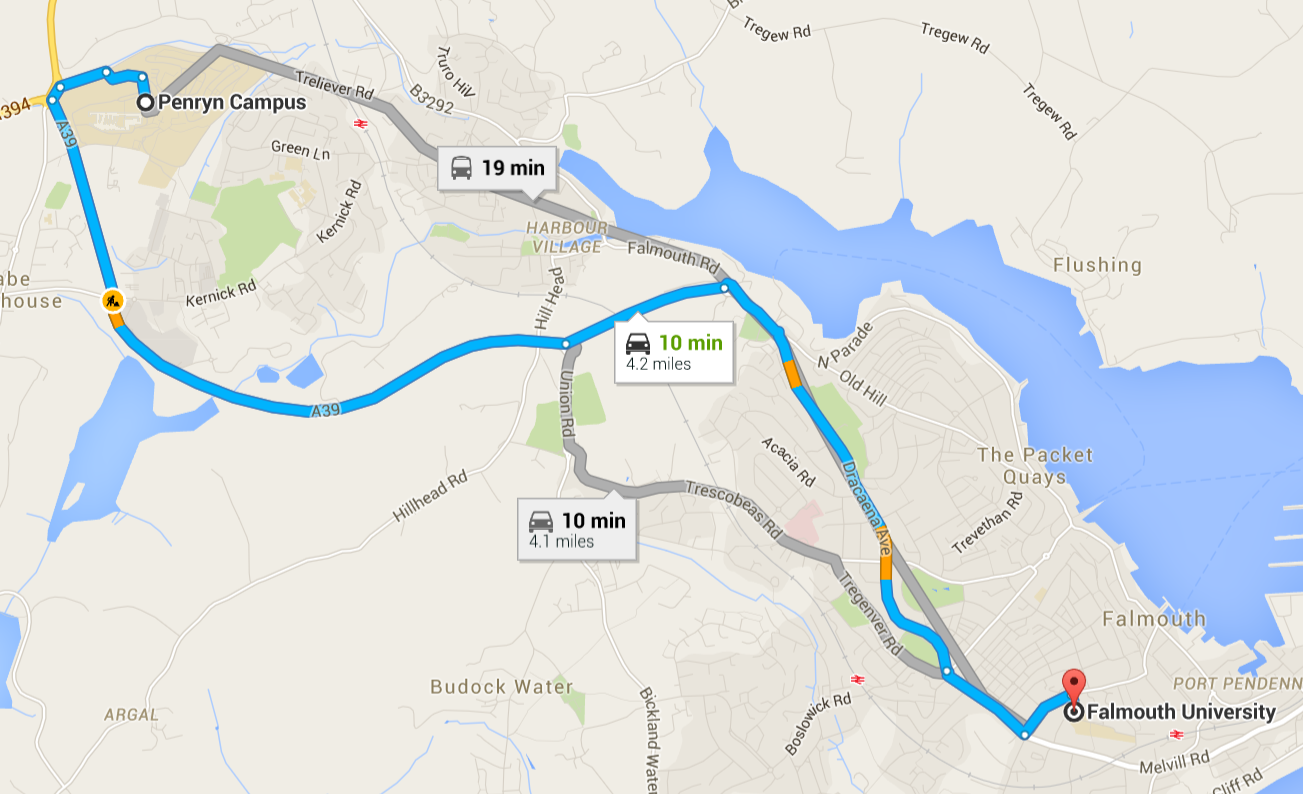
\includegraphics[width=\textwidth]{pathfinding_1}
    \end{center}
\end{frame}

\begin{frame}{Applications of pathfinding}
    \begin{center}
        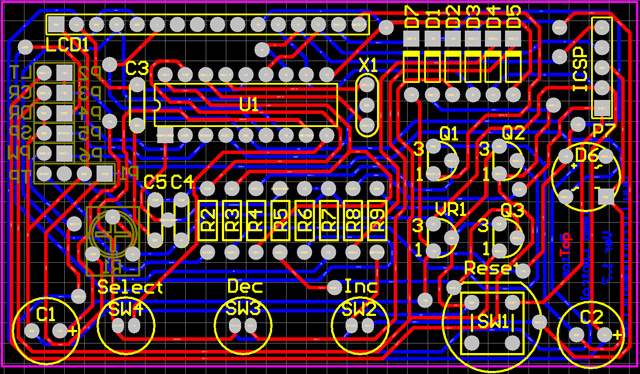
\includegraphics[width=\textwidth]{pcb}
    \end{center}
\end{frame}

\begin{frame}{Applications of pathfinding}
    Many applications in game AI \pause
    \begin{itemize}
        \item Non-player character AI \pause
        \item Mouse-based movement (e.g.\ strategy games) \pause
        \item Maze navigation \pause
        \item Puzzle solving
    \end{itemize}
\end{frame}

\begin{frame}{Aside: data structures}
	\begin{itemize}
		\pause\item \textbf{Stack}: can \textbf{push} to the top and \textbf{pop} from the top
			\begin{itemize}
				\pause\item ``Last in, first out''
			\end{itemize}
		\pause\item \textbf{Queue}: can \textbf{enqueue} to the back and \textbf{dequeue} to the front
			\begin{itemize}
				\pause\item ``First in, first out''
			\end{itemize}
		\pause\item \textbf{Priority queue}: maintains its elements in \textbf{sorted} order
			\begin{itemize}
				\pause\item \textbf{Enqueue} automatically puts the element in the correct position according to its priority
				\pause\item \textbf{Dequeue} gives the highest priority element currently in the queue
				\pause\item Usually implemented as a \textbf{heap} or a \textbf{balanced tree}...
				\pause\item ... but implementations are available for all popular programming languages
			\end{itemize}
	\end{itemize}
\end{frame}

\begin{frame}{Graph traversal}
	\begin{itemize}
		\pause\item \textbf{Depth-first} or \textbf{breadth-first}
		\pause\item Recall: can be implemented with a \textbf{stack} or a \textbf{queue} respectively
		\pause\item Inefficient --- generally has to explore the \textbf{entire map}
		\pause\item Finds a path, but probably not the \textbf{shortest}
	\end{itemize}
\end{frame}

\begin{frame}{Greedy search}
	\begin{itemize}
		\pause\item Always try to move \textbf{closer} to the goal
		\pause\item Can be implemented with a \textbf{priority queue}
		\pause\item Doesn't handle \textbf{dead ends} well
		\pause\item Not guaranteed to find the \textbf{shortest} path
	\end{itemize}
\end{frame}

\begin{frame}{A$^*$ search}
    \begin{itemize}
    	\pause\item Let $h(x)$ be an estimate of the distance from $x$ to the goal
    	\pause\item Let $g(x)$ be the distance of the path found from the start to $x$
    	\pause\item Choose a node that minimises $g(x) + h(x)$
		    \begin{itemize}
		    	\pause\item Contrast with greedy search, which just minimises $h(x)$
			\end{itemize}
    \end{itemize}
\end{frame}

\begin{frame}{Properties of A$^*$ search}
    \begin{itemize}
        \item A$^*$ is \textbf{guaranteed} to find the shortest path
            if the distance estimate $h(x)$ is \textbf{admissible} \pause
        \item Essentially, \textbf{admissible} means it must be an \textbf{underestimate} \pause
            \begin{itemize}
                \item E.g.\ straight line Euclidean distance is clearly an underestimate
                    for actual travel distance \pause
            \end{itemize}
        \item The more accurate $h(x)$ is, the more efficient the search \pause
            \begin{itemize}
                \item E.g.\ $h(x) = 0$ is admissible, but not very helpful \pause
            \end{itemize}
        \item $h(x)$ is a \textbf{heuristic} \pause
            \begin{itemize}
                \item In AI, a heuristic is an estimate based on human intuition \pause
                \item Heuristics are often used to prioritise search,
                    i.e.\ explore the most promising options first
            \end{itemize}
    \end{itemize}
\end{frame}

\begin{frame}{Tweaking A$^*$}
	\begin{itemize}
		\pause\item Can change how $g(x)$ is calculated
			\begin{itemize}
				\pause\item Increased movement cost for rough terrain, water, lava...
				\pause\item Penalty for changing direction
			\end{itemize}
		\pause\item Different $h(x)$ can lead to different paths (if there are multiple ``shortest'' paths)
	\end{itemize}
\end{frame}

\begin{frame}{String pulling}
	\begin{itemize}
		\pause\item Paths restricted to edges can look unnatural
		\pause\item Intuition: visualise the path as a string, then pull both ends to make it taut
		\pause\item Simple algorithm:
			\begin{itemize}
				\pause\item Found path is $p[0], p[1], \dots, p[n]$
				\pause\item If the line from $p[i]$ to $p[i+2]$ is unobstructed, remove point $p[i+1]$
				\pause\item Repeat until there are no more points that can be removed
			\end{itemize}
	\end{itemize}
\end{frame}


\part{Navigation meshes}
\frame{\partpage}

\begin{frame}{Pathfinding in videogames}
	\begin{itemize}
		\pause\item A$^*$ works on any \textbf{graph}
		\pause\item But what if the game world is not a graph? E.g.\ complex 3D environments
	\end{itemize}
\end{frame}

\begin{frame}{Waypoint navigation}
	\begin{columns}
		\begin{column}{0.4\textwidth}
			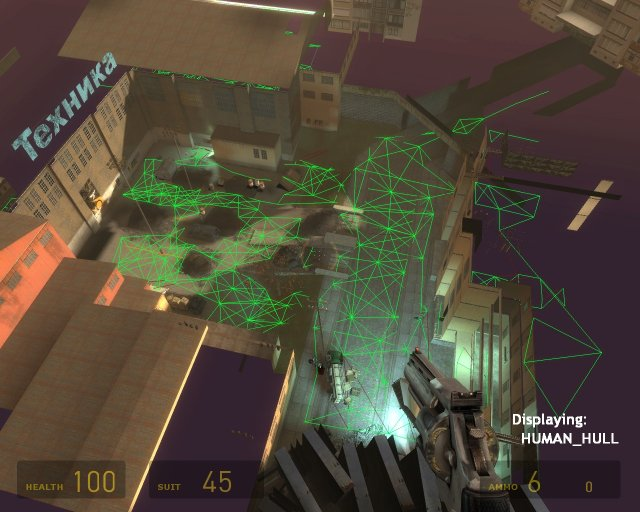
\includegraphics[width=\textwidth]{nodegraph} % https://developer.valvesoftware.com/wiki/Nodegraph
		\end{column}
		\begin{column}{0.58\textwidth}
			\begin{itemize}
				\pause\item Manually place graph nodes in the world
				\pause\item Place them at key points, e.g.\ in doorways, around obstacles
				\pause\item Works, but...
					\begin{itemize}
						\pause\item More work for level designers
						\pause\item Requires lots of testing and tweaking to get natural-looking results
						\pause\item No good for dynamic environments
					\end{itemize}
			\end{itemize}
		\end{column}
	\end{columns}
\end{frame}

\begin{frame}{Navigation meshes}
	\begin{columns}
		\begin{column}{0.4\textwidth}
			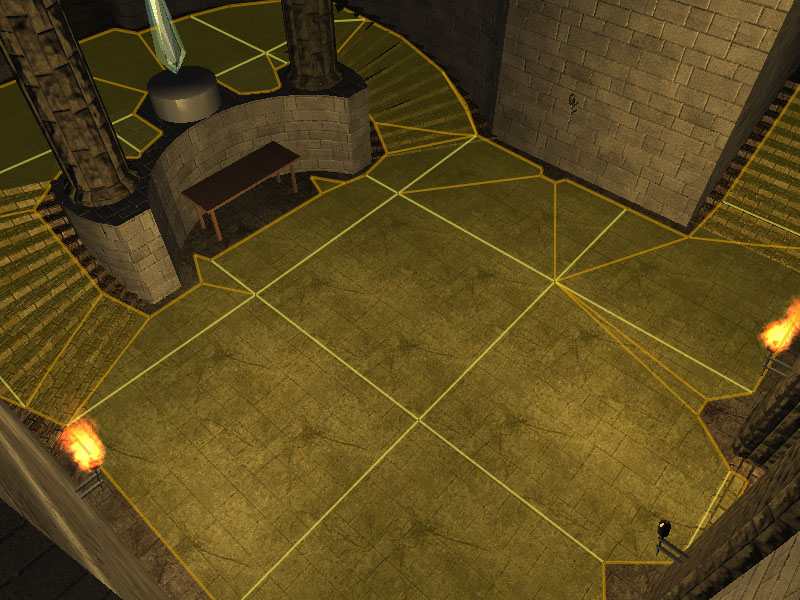
\includegraphics[width=\textwidth]{navmesh} % http://www.crystalspace3d.org/blog/leonardord?cat=53
		\end{column}
		\begin{column}{0.58\textwidth}
			\begin{itemize}
				\pause\item Automatically generate navigation graph from level geometry
				\pause\item Basic idea:
					\begin{itemize}
						\pause\item Filter level geometry to those polygons which are \textbf{passable}
							(i.e.\ floors, not walls/ceilings/obstacles)
						\pause\item Generate graph from polygons
					\end{itemize}
			\end{itemize}
		\end{column}
	\end{columns}
\end{frame}

\begin{frame}{Meshes to graphs}
	\begin{center}
		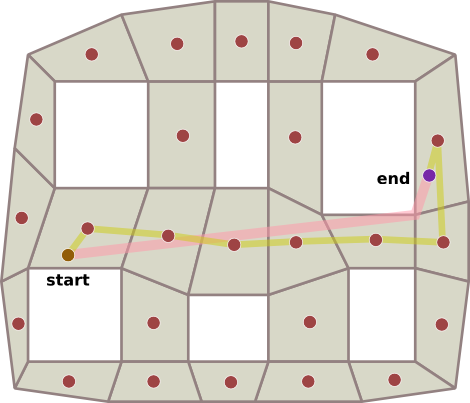
\includegraphics[width=0.6\textwidth]{polygon-navmesh-faces}
		% http://theory.stanford.edu/~amitp/GameProgramming/MapRepresentations.html
		
		Centres of polygons
	\end{center}
\end{frame}

\begin{frame}{Meshes to graphs}
	\begin{center}
		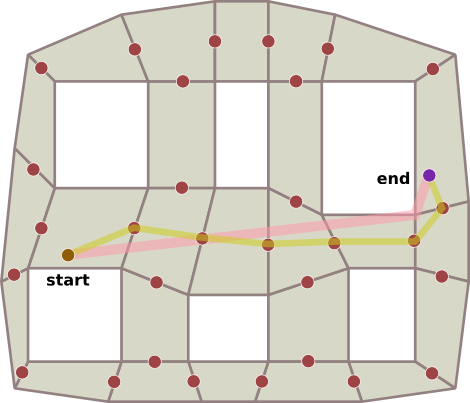
\includegraphics[width=0.6\textwidth]{polygon-navmesh-edges}
		% http://theory.stanford.edu/~amitp/GameProgramming/MapRepresentations.html
		
		Centres of edges
	\end{center}
\end{frame}

\begin{frame}{Meshes to graphs}
	\begin{center}
		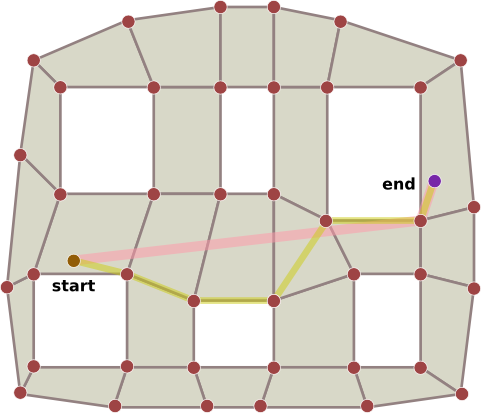
\includegraphics[width=0.6\textwidth]{polygon-navmesh-vertices}
		% http://theory.stanford.edu/~amitp/GameProgramming/MapRepresentations.html
		
		Vertices of polygons
	\end{center}
\end{frame}

\begin{frame}{Meshes to graphs}
	\begin{center}
		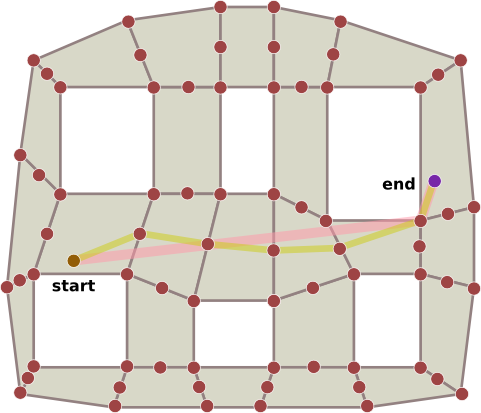
\includegraphics[width=0.6\textwidth]{polygon-navmesh-edges-and-vertices}
		% http://theory.stanford.edu/~amitp/GameProgramming/MapRepresentations.html
		
		Hybrid approach: edges and vertices
	\end{center}
\end{frame}

\begin{frame}{Following the path}
	\begin{itemize}
		\pause\item \textbf{Funnelling}: like string pulling but for navigation meshes
			\begin{itemize}
				\pause\item \url{http://digestingduck.blogspot.co.uk/2010/03/simple-stupid-funnel-algorithm.html}
				\item \url{http://jceipek.com/Olin-Coding-Tutorials/pathing.html}
			\end{itemize}
		\pause\item \textbf{Steering}: don't have your AI agent follow the path exactly, but
			instead try to stay close to it
		\pause\item \textbf{Dynamic environments}: may need to re-run pathfinder if environment changes
			(e.g.\ movable obstacles, destructible terrain)
	\end{itemize}
\end{frame}


\part{Finite state machines}
\frame{\partpage}

\begin{frame}{Finite state machines}
    \begin{itemize}
        \item A \textbf{finite state machine (FSM)} consists of: \pause
            \begin{itemize}
                \item A set of \textbf{states}; and \pause
                \item \textbf{Transitions} between states \pause
            \end{itemize}
        \item At any given time, the FSM is in a \textbf{single state} \pause
        \item \textbf{Inputs} or \textbf{events} can cause the FSM to transition to a different state
    \end{itemize}
\end{frame}

\begin{frame}{State transition diagrams}
    \begin{center}\scalebox{0.8}{
        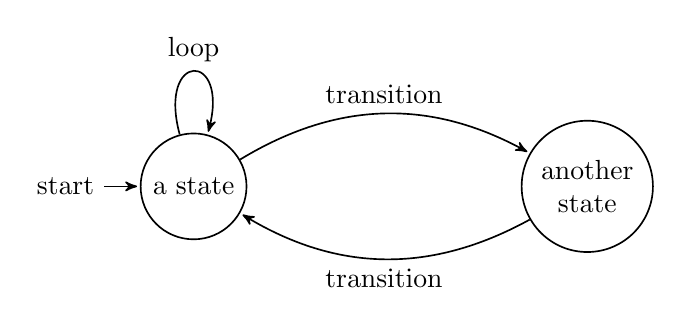
\begin{tikzpicture}[->,>=stealth',shorten >=1pt,auto,node distance=5cm,
                            semithick]
            \node[initial,state] (A) {a state};
            \node[state] (B) [right of=A, align=center] {another\\state};

            \path (A) edge [bend left] node [above] {transition} (B)
                  (B) edge [bend left] node [below] {transition} (A)
                  (A) edge [loop above] node {loop} (A);
        \end{tikzpicture}
    }\end{center}
    \begin{itemize}
        \item FSMs are often drawn as \textbf{state transition diagrams}
        \item Reminiscent of \textbf{flowcharts} and certain types of \textbf{UML diagram} \pause
    \end{itemize}
\end{frame}

\begin{frame}{FSMs for AI behaviour}
    The next slide shows a simple FSM for the following AI behaviour, for an enemy NPC in a shooter game: \pause
    \begin{itemize}
        \item By default, patrol (e.g.\ along a preset route) \pause
        \item If the player is spotted, attack them \pause
        \item If the player is no longer visible, resume patrolling \pause
        \item If you are low on health, run away and find a medikit. Then resume patrolling \pause
        \item If you are low on ammo, run away and find ammo. Then resume patrolling \pause
    \end{itemize}
\end{frame}

\begin{frame}
    \begin{center}\scalebox{0.8}{
        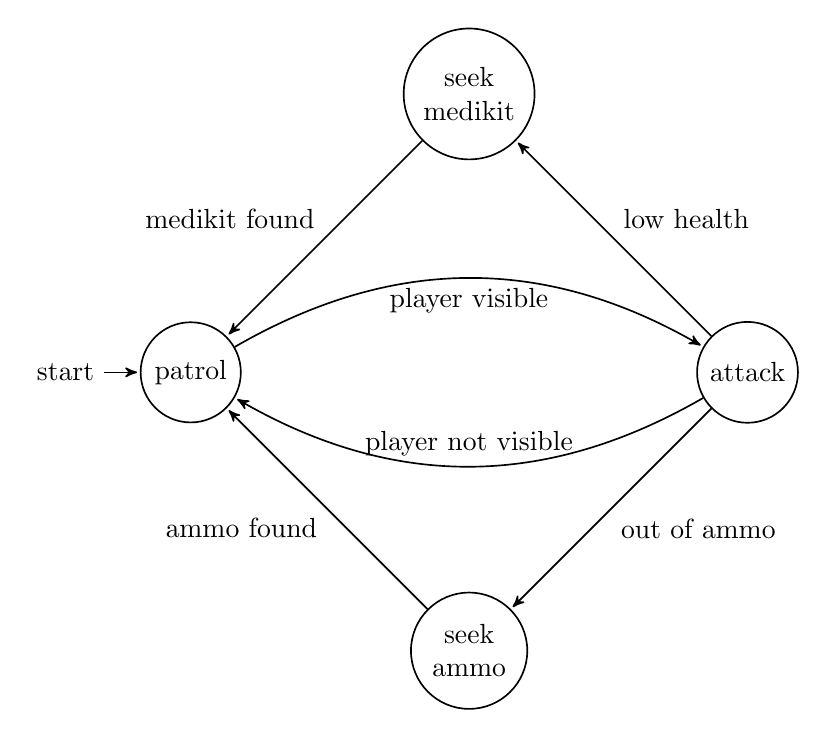
\begin{tikzpicture}[->,>=stealth',shorten >=1pt,auto,node distance=5cm,
                            semithick]
            \node[initial,state] (patrol) {patrol};
            \node[state] (health) [above right of=patrol, align=center] {seek\\medikit};
            \node[state] (ammo) [below right of=patrol, align=center] {seek\\ammo};
            \node[state] (attack) [above right of=ammo] {attack};

            \path (patrol) edge [bend left] node [below] {player visible} (attack)
                  (attack) edge [bend left] node [above] {player not visible} (patrol)
                  (attack) edge node [above right] {low health} (health)
                  (attack) edge node {out of ammo} (ammo)
                  (health) edge node [above left] {medikit found} (patrol)
                  (ammo) edge node {ammo found} (patrol);
        \end{tikzpicture}
    }\end{center}
\end{frame}

\begin{frame}{Other uses of FSMs}
    As well as AI behaviours, FSMs may also be used for: \pause
    \begin{itemize}
        \item UI menu systems \pause
        \item Dialogue trees \pause
        \item Token parsing \pause
        \item ...
    \end{itemize}
\end{frame}

\begin{frame}{Beyond FSMs}
    Some topics for you to research, for when plain old FSMs aren't enough... \pause
    \begin{itemize}
        \item Hierarchical FSMs
        \item Nested FSMs
        \item Stack-based FSMs
        \item Hierarchical task networks
        \item ...
    \end{itemize}
		Plus the topic we will be looking at today: \textbf{behaviour trees}
\end{frame}

\part{Behaviour Trees}
\frame{\partpage}

\begin{frame}{Behaviour trees (BTs)}
	\begin{itemize}
		\pause\item A \textbf{hierarchical} model of decision making
		\pause\item Allow \textbf{complex behaviours} to be built up from \textbf{simple components}
		\pause\item Allow for \textbf{more complex} behaviours than FSMs
		\pause\item First used in Halo 2 (2005), now used extensively
		\pause\item Also used in robotics and other non-game AI applications
	\end{itemize}
\end{frame}

\begin{frame}{Using BTs}
	\begin{itemize}
		\pause\item Fairly easy to implement; plenty of resources online
		\pause\item Some engines (e.g.\ Unreal) have BTs built in
		\pause\item We will be using the free \textbf{Behaviour Machine} library for Unity
	\end{itemize}
\end{frame}

\begin{frame}{BT basics}
	\begin{itemize}
		\pause\item A BT is a \textbf{tree} of \textbf{nodes}
		\pause\item On each game update (i.e.\ each frame), the root node is \textbf{ticked}
			\begin{itemize}
				\pause\item When a node is ticked, it might cause some or all of its \textbf{children} to tick as well
				\pause\item So ticks propagate down the tree from the root
			\end{itemize}
		\pause\item A ticked node returns one of three \textbf{statuses}:
			\begin{itemize}
				\pause\item Success
				\pause\item Running
				\pause\item Failure
			\end{itemize}
		\pause\item ``Running'' status allows nodes to represent operations that \textbf{last multiple frames}
	\end{itemize}
\end{frame}

\begin{frame}{Node types}
	\begin{itemize}
		\pause\item There are \textbf{three main types} of BT node
		\pause\item \textbf{Leaf} nodes
			\begin{itemize}
				\pause\item No children
				\pause\item Represent actions (i.e.\ the AI agent actually doing something)
			\end{itemize}
		\pause\item \textbf{Decorator} nodes
			\begin{itemize}
				\pause\item One child
				\pause\item Modify the execution of the child
			\end{itemize}
		\pause\item \textbf{Composite} nodes
			\begin{itemize}
				\pause\item Control which of the children are executed on each tick
			\end{itemize}
	\end{itemize}
\end{frame}

\begin{frame}{Leaf nodes}
	\begin{itemize}
		\pause\item Represent \textbf{atomic actions}
			\begin{itemize}
				\pause\item I.e.\ actions which can't sensibly be broken down into smaller actions
			\end{itemize}
		\pause\item E.g.\ walk to, crouch, attack, open door
		\pause\item Status:
			\begin{itemize}
				\pause\item Success means ``the action is done''
				\pause\item Failure means ``the action cannot be done''
				\pause\item Running means ``the action is still in progress''
			\end{itemize}
		\pause\item Leaf nodes can also be used to represent \textbf{conditions}
			\begin{itemize}
				\pause\item E.g.\ ``is my health below 10\%?''
				\pause\item Returns success for true, failure for false
			\end{itemize}
		\pause\item Leaf nodes often have \textbf{parameters} to allow for reuse in different situations
	\end{itemize}
\end{frame}

\begin{frame}[fragile]{Leaf node example}
	\begin{lstlisting}[basicstyle=\tiny\ttfamily]
using UnityEngine;
using System.Collections;
using BehaviourMachine;

public class GoTo : ActionNode
{
    public GameObjectVar objectToMove;
    public Vector3Var target;
    public FloatVar speed;

    public override Status Update()
    {
        float distance = (objectToMove.Value.transform.position - target.Value).magnitude;
        float step = speed.Value * Time.deltaTime;
        if (distance < step)
        {
            objectToMove.Value.transform.position = target.Value;
            return Status.Success;
        }
        else
        {
            objectToMove.Value.transform.position = Vector3.MoveTowards(objectToMove.Value.transform.position, target.Value, step);
            return Status.Running;
        }
    }
}
	\end{lstlisting}
\end{frame}

\begin{frame}{Composite nodes: sequence}
	\begin{itemize}
		\pause\item Run each child, in order
		\pause\item If \textbf{any} child returns failure, stop and return failure
		\pause\item If \textbf{all} children return success, stop and return success
	\end{itemize}
	\pause
	{\footnotesize\Tree
		[.\fbox{Sequence}
			[.\fbox{Walk to chest} ]
			[.\fbox{Open chest} ]
			[.\fbox{Pick up loot} ]
			[.\fbox{Close chest} ]
		]
	}
\end{frame}

\begin{frame}{Sequence nodes and conditions}
	\begin{itemize}
		\pause\item A sequence node can be used like an \lstinline{if (cond1 && cond2)} statement
	\end{itemize}
	\pause
	{\footnotesize\Tree
		[.\fbox{Sequence}
			[.\fbox{Is health $< 10$?} ]
			[.\fbox{Am I near cover?} ]
			[.\fbox{Move to cover} ]
			[.\fbox{Use medkit} ]
		]
	}
\end{frame}

\begin{frame}{Composite nodes: selector}
	\begin{itemize}
		\pause\item Run each child, in order
		\pause\item If a child returns failure, move onto the next one
		\pause\item If \textbf{any} child returns success, stop and return success
	\end{itemize}
	\pause
	{\footnotesize\Tree
		[.\fbox{Selector}
			[.\fbox{Open chest} ]
			[.\fbox{Sequence}
				[.\fbox{Unlock chest} ]
				[.\fbox{Open chest} ]
			]
			[.\fbox{Smash chest} ]
		]
	}
\end{frame}

\begin{frame}{Selectors and priority}
	\begin{itemize}
		\pause\item Order of selector children represents the \textbf{priority} of different alternatives
	\end{itemize}
	\pause
	{\scriptsize\Tree
		[.\fbox{Selector}
			[.\fbox{Sequence}
				[.\fbox{Health $<$ 10?} ]
				[.\fbox{Run away} ]
			]
			[.\fbox{Sequence}
				[.\fbox{Player visible?} ]
				[.\fbox{Attack} ]
			]
			[.\fbox{Patrol} ]
		]
	}
\end{frame}

\begin{frame}{Sequence vs selector}
	\begin{itemize}
		\pause\item Sequence: perform a list of actions; if one of them fails then abandon the task
		\pause\item Selector: try a list of alternatives; stop once you find one that works
		\pause\item Sequence works like \lstinline{and}, selector works like \lstinline{or}
	\end{itemize}
\end{frame}

\begin{frame}{Other composite nodes}
	\begin{itemize}
		\pause\item Execute children in \textbf{random} order
		\pause\item Execute children in \textbf{parallel}
		\pause\item Most BT frameworks allow programmers to create custom composite nodes
	\end{itemize}
\end{frame}

\begin{frame}{Decorator nodes}
	\begin{itemize}
		\pause\item \textbf{Inverter}: if child returns success then return failure, and vice versa
		\pause\item \textbf{Repeater}: run the child a number of times, or forever
		\pause\item Most BT frameworks allow programmers to create custom decorator nodes
	\end{itemize}
\end{frame}

\begin{frame}{Blackboard}
	\begin{itemize}
		\pause\item It is often useful to \textbf{share} data between nodes
		\pause\item A \textbf{blackboard} (sometimes called a \textbf{data context}) allows this
		\pause\item Blackboard defines \textbf{variables}, which can be \textbf{read} and \textbf{written} by nodes
		\pause\item Blackboard can be \textbf{local} to the AI agent, \textbf{shared} between several agents, or \textbf{global} to all agents
		\pause\item (Shared blackboards mean that your AI has ``telepathy'' --- this may or may not be desirable!)
	\end{itemize}
\end{frame}

\begin{frame}{BTs in The Division}
	\begin{center}
		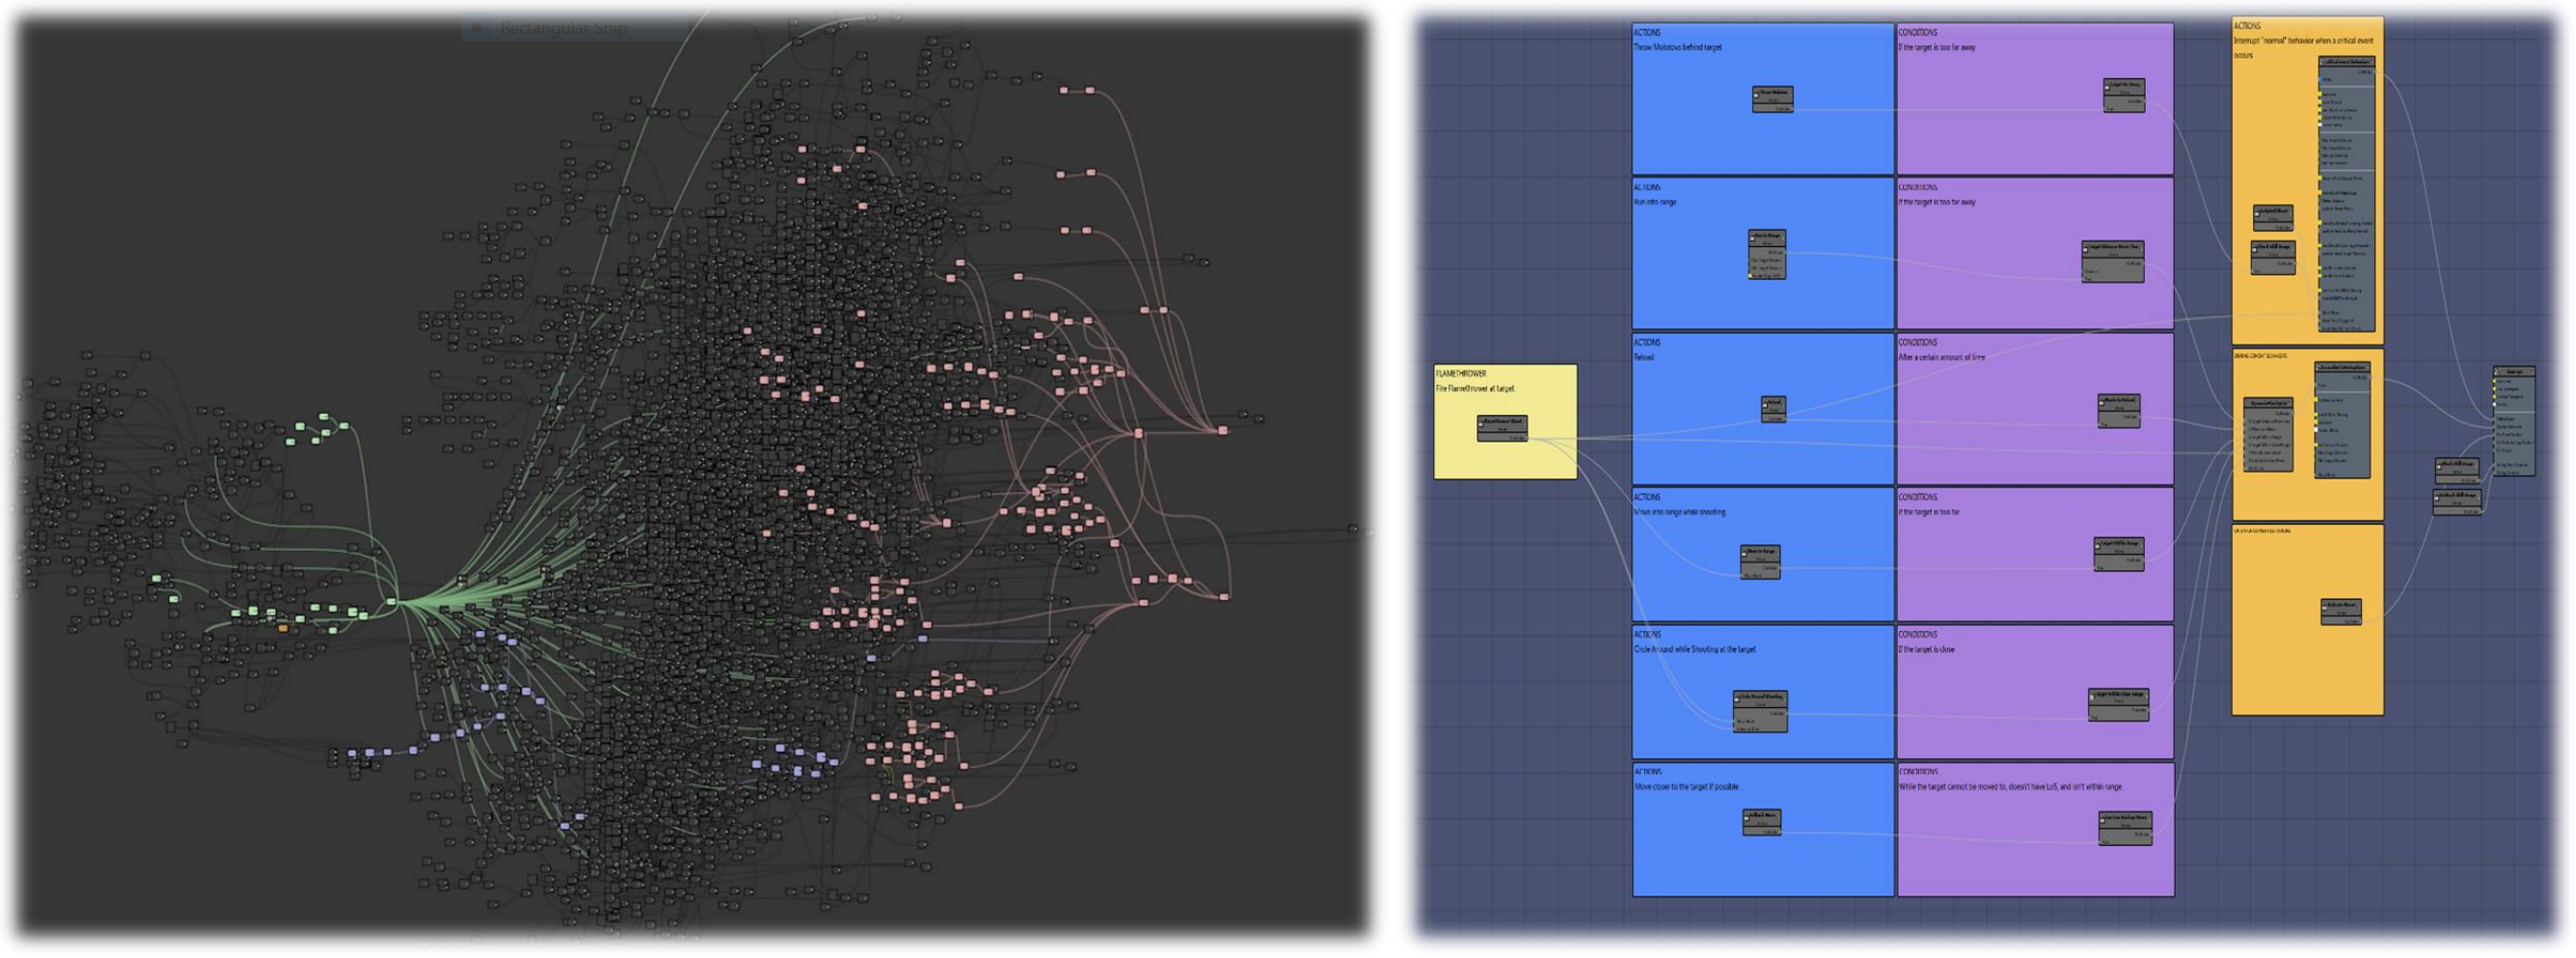
\includegraphics[width=\textwidth]{the_division}
		
		\url{http://www.gdcvault.com/play/1023382/AI-Behavior-Editing-and-Debugging}
	\end{center}
\end{frame}


\begin{frame}{Exercise}
\begin{itemize}
	\item Using FSM or Behaviour Trees, create an AI agent which does the following
	\begin{itemize}
		\item Navigates a series of waypoints
		\item Shoots at the player when in range
		\item When low on health it attempts to heal by collecting an item
	\end{itemize}
	\item Stretch Goal: Make an AI Agent to replace the player!
\end{itemize}
\end{frame}

\begin{frame}{Further Reading 1}
	\begin{itemize}
		\item Finite State AI in Unity - \url{https://unity3d.com/learn/tutorials/topics/navigation/finite-state-ai-delegate-pattern}
		\item Using Unity Animator as an FSM - \url{https://medium.com/the-unity-developers-handbook/dont-re-invent-finite-state-machines-how-to-repurpose-unity-s-animator-7c6c421e5785}
		\item Behaviour Machine (FSM \& BT for Unity) - \url{http://www.behaviourmachine.com/}
		\item Unity Behavior Library - \url{https://github.com/listentorick/UnityBehaviorLibrary/}
		\item Unity Crystal AI - \url{https://igiagkiozis.github.io/CrystalAI/}
	\end{itemize}
\end{frame}

\begin{frame}{Further Reading 2}
\begin{itemize}
	\item Behaviour Trees in Project Zomboid - \url{https://www.gamasutra.com/blogs/ChrisSimpson/20140717/221339/Behavior_trees_for_AI_How_they_work.php}
	\item Behaviour Trees in Unreal - \url{https://docs.unrealengine.com/latest/INT/Engine/AI/BehaviorTrees/QuickStart/}
\end{itemize}
\end{frame}
\end{document}